\section{Semantic Parsing}

\subsection*{Definition}
Parse of meaning. Represented by logical form composed of variables, predicates, quantifiers and boolean. Example: $\forall p .(P e r s o n(p) \rightarrow \exists q .(P e r s o n(q)$
$\wedge p \neq q \wedge \operatorname{Loves}(p, q)))$.

\subsection*{Principle of Compositionality}
The meaning of a complex expression is a function of
the meanings of that expression's constituent parts.

\subsection*{Enriched lambda calculus to represent meanings}

(1) Logical constants such as entities (e.g., ALEX) and relations (e.g., likes). 
(2) Variables, which are undetermined objects, similar to free variables in lambda calculus.
(3) Literals such as LIKES(ALEX, x), formed by applying relations to objects.
(4) Logical terms built using literals with logical connectives (e.g., $\land$) and quantifiers (e.g., $\exists$).
(5) lambda terms built using lambda operator.

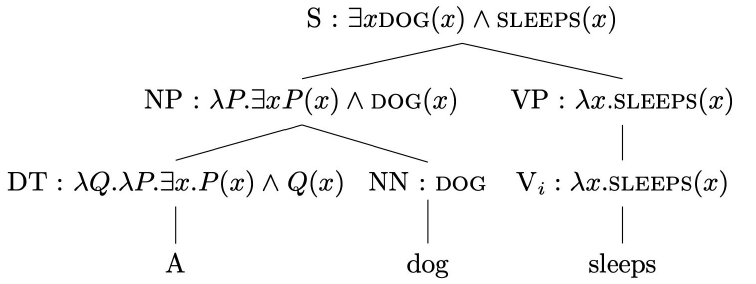
\includegraphics[width=.22\textwidth]{img/semantic_representation.png}
